\section{Overview of the proposed framework to obtain training videos}
\label{sec:overview}

In this section, we provide an overview of our proposed framework and approaches for identifying and selecting keywords to obtain training videos with the two desired properties described in Section~\ref{sec:desiredpropdata}. 

\indent   As discussed in Section~\ref{sec:intro}, obtaining training videos for arbitrary set of categories through manual effort is not scalable to large sizes of training data. Training videos could alternatively be obtained in an automated manner using a video search engine. This approach has also been briefly mentioned in \cite{wang2010youtubecat}, to obtain weakly labeled videos. Let $RV(K)$ represent the set of retrieved videos obtained by querying keyword $K$ in a video search engine, such as YouTube~\cite{Youtube} or Vimeo~\cite{Vimeo}. The training videos of category $i$, i.e., $T(i)$ can then be obtained simply as $RV(C_i)$, where $C_i$ is the name of category $i$. Though simple, this technique has few shortcomings. It focuses only on occurrence of the name of category and not on its semantic meaning. For example $RV(\text{`}Baby\text{'})$ mainly retrieves videos on funny kids, and music videos or other popular videos containing the word `Baby' in their title or tags. As a result, there are several mislabeled videos among training videos obtained by this approach. In Section~\ref{sec:expt}, we show how this leads to poor performance as more videos are retrieved just by the category name. At the same time, this approach does not cover the many of the semantic topics that we associate with the category of concern. For the category $Baby$, these include topics such as (in addition to funny kids,) Strollers and Bassinets reviews, Babysitting tutorials, Newborn care, Pregnancy, and several others (Fig.~\ref{fig:trainingdatapropsfigs}(b)). The Intra-Category Diversity by such an approach is hence quite low, leading to poor classifier performance. Through the proposed framework, we attempt to address the above shortcomings. We use the training videos obtained by querying name of category, i.e., $T(i)=RV(C_i)$, to train baseline classifiers to compare with our proposed approach. 

\subsection{Overview of proposed framework}
\label{sec:overviewframework}

In the proposed framework, we first collect several keywords that are related to the name of category ($C_i$). These comprise the \textbf{Candidate Keywords}. The Candidate Keywords (called candidates for brevity) can be obtained on the basis of correlation or co-occurrence with the name of the category from publicly available text documents (such as Wikipedia). Thesauri~\cite{nakayama2007wikipedia} also provide a good source for semantically (i.e., in terms of meaning) similar keywords, and can be used to obtain candidates. In addition, candidates can be obtained as related concepts or keywords from sources such as~\cite{ReverseDictionary}. The candidates can be queried in a video search engine, and their retrieved videos can be collected to obtain T($i$). However some candidates would be more useful than others, and some might be outright harmful, if used to retrieve training videos for category $i$. We discuss this in the next section. On the basis of a proposed keyword selection algorithm, we select a subset of keywords from a set of candidates for category $i$. The Selected Retriever Keywords (or SRKs) thus selected are used to retrieve training videos. If \{$K_{i,1}, K_{i,2}, ... , K_{i,L}$\}  are the SRKs for category $i$, then the training data for category $i$, i.e., $T(i)$, can be obtained as:
\begin{equation} \label{eq:trainingDataUnioneqn}
\indent T(i) = \left [ \bigcup_{j=1}^{L}RV(K_{i,j}) \right ]\cup RV(C_{i}). 
\end{equation}

If $T(i)$ were obtained as per (\ref{eq:trainingDataUnioneqn}) by selecting any arbitrary candidate keywords of category $i$ as SRKs, then $T(i)$ may not necessarily have the desired properties discussed in Section~\ref{sec:desiredpropdata}, namely low mislabeled videos, and high Intra-Category Diversity. In the next section, we discuss how we can determine the suitability of candidates to retrieve training videos with the desired properties discussed in Section~\ref{sec:desiredpropdata}.  

\subsection{Selection Procedure for Selected Retriever Keywords (SRKs)}
\begin{figure}
\centering
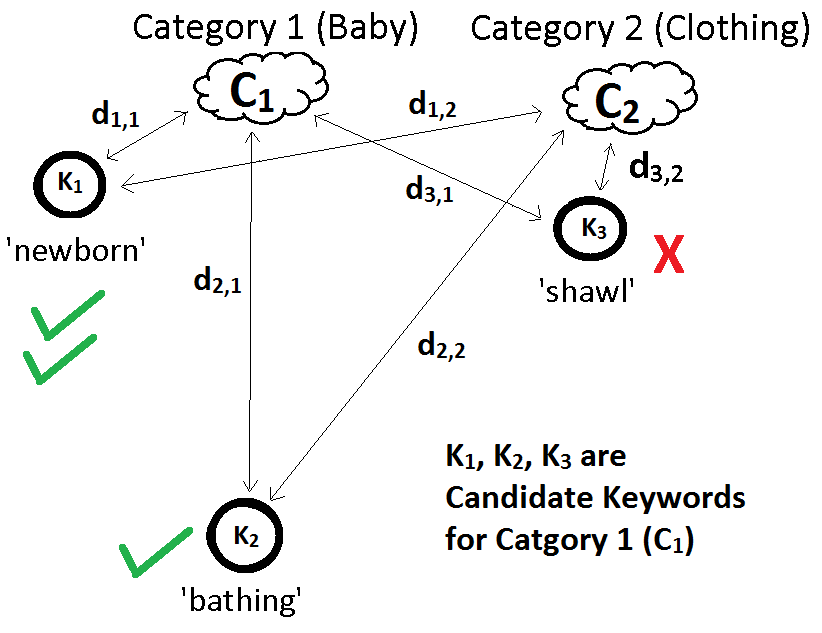
\includegraphics[width=0.6\linewidth]{TrainingData/WIfigures/keyword_properties_Baby2.png}
\caption{Selection criteria for Selected Retriever Keywords}
\label{fig:KeywordProperties}
\end{figure}

\label{sec:overviewselectSRK}
\begin{figure*}[htb!]
\centering
\begin{tabular}{cc}
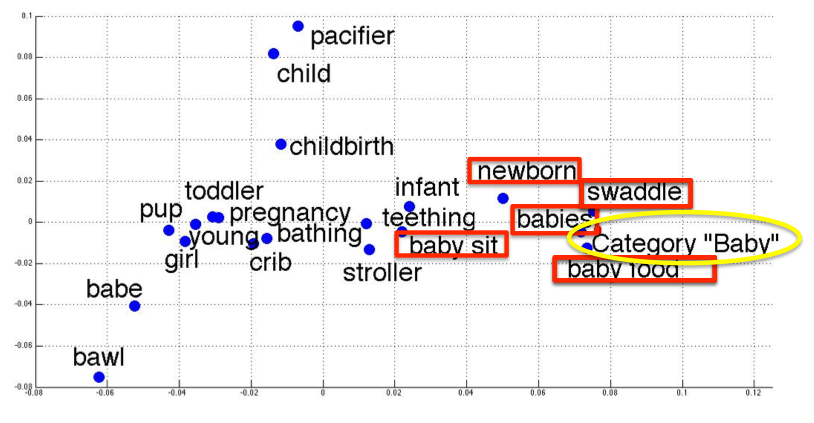
\includegraphics[width=0.47\textwidth,clip=]{TrainingData/figs/Baby_20_5_proxKwds.png} & 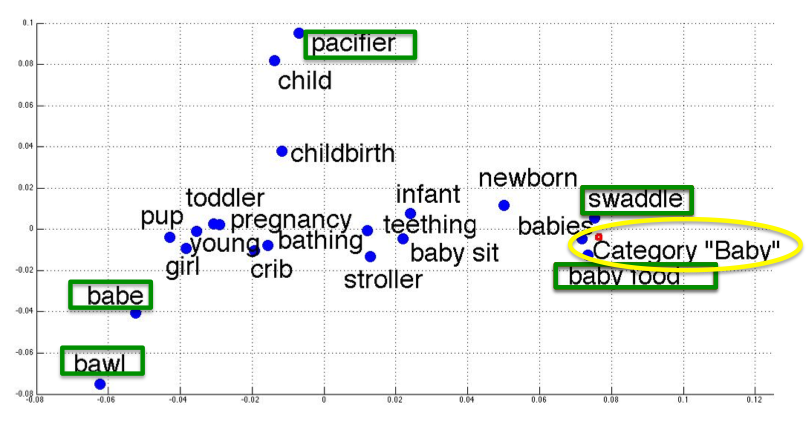
\includegraphics[width=0.47\textwidth,clip=]{TrainingData/figs/Baby_20_5_DiverseKwds.png}\\ 
(a) & (b) \\ 
\end{tabular}
\caption{\small{For a set of 20 valid keywords for the category `$Baby$', (a) shows the 5 most proximate keywords and (b) shows the 5 most diverse keywords. Diversity is measured as outlined in Section~\ref{sec:aao}. As can be seen, the set of keywords optimizing either objective function are very different from each other. Note that in order to plot the keywords on a graph, the first two dimensions obtained from principal component analysis (PCA)~\cite{jolliffe2002principal} are used. }}
\label{fig:proxdivkwdBabyExamplePCA}
\end{figure*}

Before we discuss suitability of candidates, and the selection procedure for SRKs, we provide the following result to help in our discussions. Consider the set of categories $\{i\}_{i=1}^{N_{Cat}}$, where each category $i$ is a multivariate normal distribution with mean $\mu_i$. Assume that the set of videos across all categories (referred to as data) is whitened, i.e., has uncorrelated dimensions of variance unity. Then $\Sigma_i = I$, i.e., the covariance matrices for all categories reduce to an identity matrix. Under assumptions of equiprobable categories, we derive that a video (represented as $v$) belongs to category $\hat{i}$ iff 
\begin{equation*} 
\hat{i}=\argmax_i{e^{-\frac{(v - \mu_i)^{T}\Sigma_i (v - \mu_i) }{2} }} \text{ , i.e., iff }
\end{equation*}
\begin{equation*} 
\hat{i}=\argmin_i{e^{ \mid v - \mu_i \mid ^{2}  }} \text{ , i.e., iff }
\end{equation*}
\begin{equation} \label{eq:proof6}
\hat{i}=\argmin_i{\mid v-\mu_i\mid}.
\end{equation}

Here $\mu_i$ is the mean of category $i$, as determined by an oracle. $ \mid v - \mu_i \mid$ is the Euclidean distance between $v$ and $\mu_i$. Note that for this chapter, $v$ is represented as a bag of words~\cite{salton1975vector} vector based on the contextual information surrounding $v$. On the basis of the above assumptions, and using (\ref{eq:proof6}), a keyword $K$ retrieves more videos having true label as category $i$ than videos having true label as category $j ( \neq  i)$ if
\comment{
\begin{multline} \label{eq:proof7}
\sum_{v:v\in RV(K)}\mathcal{I}(\argmin_l{\mid v-\mu_l \mid}=i) \; \; \; > \\
\indent \sum_{v:v\in RV(K)}\mathcal{I}(\argmin_l{\mid v-\mu_l \mid}=j) \; \;  \forall j \neq i.
\end{multline}
}
\begin{equation}
\sum_{v:v\in RV(K)}\mathcal{I}(\argmin_l{\mid v-\mu_l \mid}=i) > \sum_{v:v\in RV(K)}\mathcal{I}(\argmin_l{\mid v-\mu_l \mid}=j)  \forall j \neq i.
\label{eq:proof7}
\end{equation}

Here, $\mathcal{I}(.)$ is an indicator function that is $1$ if its argument is true, and $0$ if its argument is false. $\mu_l$ is the true mean of category $l$. In (\ref{eq:proof7}), the closest category for each video in $RV(K)$ is obtained, in terms of Euclidean distance. Checking (\ref{eq:proof7}) for a keyword $K$ thus has complexity $O( \mid RV(K) \mid.N_{Cat})$, where $N_{Cat}$ is the number of categories, and $\mid RV(K) \mid$ is the cardinality of the set $RV(K)$. In order to reduce the above high complexity, (\ref{eq:proof7}) can be approximated by obtaining the closest category of centroid of the set $RV(K)$. This reduces the complexity to $O(N_{Cat})$. For category $i$, we define \textbf{Valid Candidate Keywords} (called valid keywords for brevity) as those Candidate Keywords that retrieve more videos having true label of category $i$ than of any other category. Then for a candidate $K$ of category $i$, $K$ is a valid keyword if 
\begin{equation} \label{eq:ValidityFilter}
\mid \mu_K - \mu_i \mid < \mid \mu_K - \mu_j \mid \forall j \neq i. 
\end{equation}
Here $\mu_K$ =  $\frac{ \sum{v:v \in RV(K)} }{\mid RV(K) \mid}$. The true mean $\mu_i$ for category $i$ can be approximated as centroid of $RV(C_i)$, i.e., of the set of videos retrieved by name of category $i$. Equation (\ref{eq:ValidityFilter}) is called the \textbf{Validity Filter}. Only valid keywords should be considered for being selected as SRK to ensure more number of training videos are added in $T(i)$ that have true label of category $i$ than videos that are mislabeled as category $i$. 

Note that we have assumed that the data generating the above distributions is whitened. If the given data is not whitened, its dimensions can be rotated into space of principal components, and each dimension divided by square root of variance in that dimension, in order to whiten the data. Also, if the assumption that categories are equiprobable multivariate normal distributions does not hold, then the exact distributions could be used to derive the Validity Filter as shown in (\ref{eq:ValidityFilter}). As a result, the complexity of checking the validity of a keyword may be more than $O(N_{Cat})$, however our approach of using a Validity Filter, and the following keyword selection procedure would still be valid. We continue our discussion with the above assumption. 

Let us consider the scenario shown in Fig.~\ref{fig:KeywordProperties}. Keywords $K_1$, $K_2$, $K_3$ are candidates for category $1$ ($C_1$). $K_3$, as can be seen, is closer in terms of Euclidean distance, to category $2$ ($C_2$) than to $C_1$, and hence fails the Validity Filter (\ref{eq:ValidityFilter}). For $C_1$ and $C_2$ as $Baby$ and $Clothing$ respectively, example keywords (from actual data) for $K_1$, $K_2$, $K_3$ are `$newborn$', `$bathing$',  `$shawl$' respectively. Note that a candidate may have a weak semantic relationship with its corresponding category name. For example, the candidates' source \cite{ReverseDictionary} recommends `$shawl$' as a candidate keyword for $Baby$ category since they are related perhaps owing to the use of shawls to cover or carry babies with. 
However querying `$shawl$' ($K_3$) in a video search engine is much less likely to retrieve $Baby$ related videos than it is to retrieve $Clothing$ related videos. Thus including $RV(`shawl\text{'})$ in training data of category $Baby$ would add more mislabeled videos in $T(Baby)$ than videos having true label of category $Baby$. Validity Filter (\ref{eq:ValidityFilter}) ensures that candidates such as `$shawl$' are not valid keywords for category $Baby$. 

Let $N_{Valid,i}$ be the number of valid keywords for category $i$. In order to select keywords form the valid keywords, we determine the suitability of keywords to retrieve training videos for category $i$ based on two components: 1) High Proximity, 2) High Diversity. We discuss below how the above components lead to training videos having the desired properties, less mislabeled videos and high Intra-Category Diversity respectively.  


\textbf{\textit{High Proximity.}} Under assumptions of whitened data and multivariate normal distributions as the categories, the likelihood of a video $v$ belonging to a category $i$ is proportional to $e^{(-\frac{1}{2}\mid v-\mu_i \mid^2)}$. Assuming equal prior probabilities for all categories, the probability that $v$ has its true label as category $i$ is higher when $\mid v - \mu_i \mid$ is lower, where $\mu_i$ is the true mean of category $i$. Thus, if $v$ is a video in training data of category $i$, then P(\textit{v is a mislabeled video}) is lower when $\mid v - \mu_i \mid$ is lower. Consider a valid keyword $K$ for category $i$. Satisfying (\ref{eq:ValidityFilter}) merely implies that $RV(K)$ contains more videos of true label category $i$ than videos that are mislabeled as category $i$. Preference should be given to valid keywords that lead to lesser mislabeled videos in the resulting set of training videos of category $i$. In order to do so, a valid keyword $K$ should be preferred if the videos in $RV(K)$ are closer to $\mu_i$. We thus calculate \textbf{Proximity score} for each valid keyword $K$ as 
\begin{equation} \label{eq:proximityscore}
\text{Proximity score for $K$}= \{ 1/\mid \mu_K - \mu_i \mid \}, 
\end{equation}
 where $\mu_K$ is the centroid of $RV(K)$. A keyword $K$ should be preferred to be selected as a Selected Retriever Keyword (SRK) if the Proximity Score of $K$ is high.  

In Fig.~\ref{fig:KeywordProperties}, `$newborn$' ($K_1$) and `$bathing$' ($K_2$) are both Valid Candidate Keywords for category $Baby$ ($C_1$). Since the centroid of $RV(\text{`}newborn\text{'})$ is closer to the mean of $C_1$ than the centroid of $RV(\text{`}bathing\text{'})$, the proximity score of `$newborn$' is more than that of `$bathing$'. Thus as per the proximity score, the valid keyword `$newborn$' should be preferred over `$bathing$'. Since \textit{P(true label of $v =C_1 \mid  v \in RV(\text{`}newborn\text{'})$)} is more than \textit{P(true label of $v =C_1 \mid  v \in RV(\text{`}bathing\text{'})$)}, preferring `$newborn$' over `$bathing$' as SRK reduces mislabeled videos in resulting set of training videos.  

Note that the measurement of Proximity score of a valid keyword is the same for both approaches proposed in Section~\ref{sec:overviewselectSRK}. 

\textbf{\textit{High Diversity.}} Intuitively, the diversity of a set of keywords reflects the Intra-Category Diversity of the set of videos that are retrieved using the keywords. For the LCPD approach discussed next in Section~\ref{sec:lcpd}, the Intra-Category Diversity of the training videos of category $i$, i.e., $div(T(i))$ is measured based on variance of the set of videos $T(i)$. Based on such a measure for $div(T(i))$, a diversity score can be defined for each keyword $K$ given a subset of the training data of category $i$, denoted by $T\text{'}(i)$. Details of such a \textit{per-keyword} measurement of Intra-Category Diversity are provided in Section~\ref{sec:lcpd}. As an alternative way, since training videos are retrieved using SRKs, the degree of variation in $T(i)$ could also be estimated based on the degree of variation in the set of keywords that are used to obtain them. Based on this insight, the second keyword selection approach (AAO approach in Section~\ref{sec:aao}) uses a diversity measure for a set of keywords, instead of a diversity measure per keyword as used in Section~\ref{sec:lcpd}. In order to obtain a diversity measure for a set of keywords, distance or linear independence based measures can be used. Section~\ref{sec:aao} discusses the efficiency implications of different diversity measures for set of keywords. For the AAO approach, we utilize linear independence based diversity measures for set of keywords. 

Based on the above discussion, SRKs need to be selected such that they have high proximity score, and high diversity. Selecting keywords based on high proximity tends to prefer keywords that retrieve videos similar or \textit{close} to those retrieved by the name of the category. On the other hand, selecting keywords based on high diversity tends to prefer keywords that are more different or \textit{far} from each other. Thus the two objectives tend to be opposing in nature. Figures~\ref{fig:proxdivkwdBabyExamplePCA}(a) and \ref{fig:proxdivkwdBabyExamplePCA}(b) provide an example of a set of 5 keywords selected based on either objective for a set of 20 valid keywords of the category `$Baby$'. As can be seen, the sets of keywords optimizing either objective are very different from each other and optimizing for one tends to lead to keywords having poor objective score for the other. In the next section, we propose approaches to address keyword selection problem based on such conflicting objectives. 

